%iffalse
\let\negmedspace\undefined
\let\negthickspace\undefined
\documentclass[journal,12pt,onecolumn]{IEEEtran}
\usepackage{cite}
\usepackage{amsmath,amssymb,amsfonts,amsthm}
\usepackage{algorithmic}
\usepackage{graphicx}
\usepackage{textcomp}
\usepackage{xcolor}
\usepackage{txfonts}
\usepackage{listings}
\usepackage{enumitem}
\usepackage{mathtools}
\usepackage{gensymb}
\usepackage{comment}
\usepackage[breaklinks=true]{hyperref}
\usepackage{tkz-euclide} 
\usepackage{listings}
\usepackage{booktabs}
\usepackage{pgfplots}
\usepackage{gvv}                                        
\usepackage[latin1]{inputenc}     
\usepackage{xparse}
\usepackage{color}                                            
\usepackage{array}                                            
\usepackage{longtable}                                       
\usepackage{calc}                                             
\usepackage{multirow}
\usepackage{multicol}
\usepackage{hhline}                                           
\usepackage{ifthen}                                           
\usepackage{lscape}
\usepackage{tabularx}
\usepackage{array}
\usetikzlibrary{patterns}
\usepackage{siunitx}
\pagestyle{empty}
\usetikzlibrary{calc}
\usepackage[margin=1in]{geometry}
\usepackage{pgffor}
\usepackage{float}
\newtheorem{theorem}{Theorem}[section]
\newtheorem{problem}{Problem}
\newtheorem{proposition}{Proposition}[section]
\newtheorem{lemma}{Lemma}[section]
\newtheorem{corollary}[theorem]{Corollary}
\newtheorem{example}{Example}[section]
\newtheorem{definition}[problem]{Definition}
\newcommand{\BEQA}{\begin{eqnarray}}
\newcommand{\EEQA}{\end{eqnarray}}
\newcommand{\define}{\stackrel{\triangle}{=}}
\theoremstyle{remark}
\newtheorem{rem}{Remark}
% Marks the beginning of the document
\pgfplotsset{compat=1.18}
\begin{document}
\bibliographystyle{IEEEtran}
\vspace{3cm}

\title{2022-ME-'40-52'}
\author{EE24BTECH11023}
%\maketitle
%\newpage
%\bigskip
\maketitle

{\let\newpage\relax\maketitle}

\renewcommand{\thefigure}{\theenumi}
\renewcommand{\thetable}{\theenumi}
\setlength{\intextsep}{10pt} % Space between text and floats


\numberwithin{equation}{enumi}
\numberwithin{figure}{enumi}
\renewcommand{\thetable}{\theenumi}

\begin{enumerate}
    \item A bracket is attached to a vertical column by means of two identical rivets $U$ and $V$ separated by a distance of $2a = 100$ mm, as shown in the figure. The permissible shear stress of the rivet material is $50$ MPa. If a load $P = 10$ kN is applied at an eccentricity $e = 3\sqrt{7}a$, the minimum cross-sectional area of each of the rivets to avoid failure is {\underline{\hspace{2cm}}} mm$^2$.
     \begin{figure}[H]
        \centering
        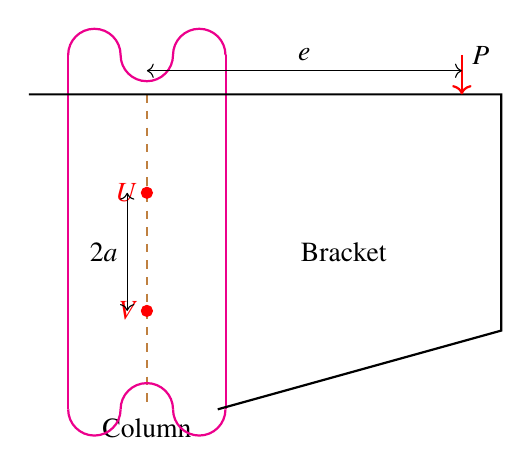
\begin{tikzpicture}
    \node[below] at (-0.5, -2) {Column};
    \draw[thick,magenta] (-1.5,2.5)--(-1.5,-2);
    \draw[thick,magenta] (0.5,2.5)--(0.5,-2);
    \draw[dashed, thick, brown] (-0.5,2) -- (-0.5,-2);
    \draw[thick] (-2,2) -- (4,2) -- (4,-1) -- (0.4,-2);
    \coordinate (A) at (-1.5,2.5);
    \coordinate (B) at (0.5,2.5);
    \draw[magenta, thick] (-0.834, 2.5) arc[start angle=0, end angle=180, radius=0.333cm];
    \draw[magenta, thick] (-0.834, 2.5) arc[start angle=-180, end angle=0, radius=0.333cm];
    \draw[magenta, thick] (0.498, 2.5) arc[start angle=0, end angle=180, radius=0.333cm];
    \draw[magenta, thick] (-1.5, -2) arc[start angle=-180, end angle=0, radius=0.333cm];
    \draw[magenta, thick] (-0.168, -2) arc[start angle=0, end angle=180, radius=0.333cm];
    \draw[magenta, thick] (-0.168, -2) arc[start angle=-180, end angle=0, radius=0.333cm];
    \draw[thick, red, ->] (3.5,2.5) -- ++(0,-0.5);
    \node[right] at (3.5,2.5) {$P$};
    \draw[<->, thin] (-0.5,2.3) -- node[above] {$e$} ++(4,0);
    \filldraw[red] (-0.5,0.75) circle (2pt) node[left] {$U$};
    \filldraw[red] (-0.5,-0.75) circle (2pt) node[left] {$V$};
    \draw[<->, thin] (-0.75,0.75) -- node[left] {$2a$} ++(0,-1.5);
    \node at (2,0) {Bracket};
\end{tikzpicture}
 
    \end{figure}   
    \begin{enumerate}
        \item $800$
        \item $25$
        \item $100\sqrt{7}$
        \item $200$
    \end{enumerate}
    \item In the Fe-Fe$_3$C phase diagram, the eutectoid composition is $0.8$ weight $\%$ of carbon at $725^\circ$ C. The maximum solubility of carbon in $\alpha$-ferrite phase is $0.025$ weight $\%$ of carbon. A steel sample, having no other alloying element except $0.5$ weight $\%$ of carbon, is slowly cooled from $1000^\circ$ C to room temperature. The fraction of pro-eutectoid $\alpha$-ferrite in the above steel sample at room temperature is:
    \begin{enumerate}
        \item 0.387
        \item 0.864
        \item 0.475
        \item 0.775
    \end{enumerate}
    \item Activities $A$ to $K$ are required to complete a project. The time estimates and the immediate predecessors of these activities are given in the table. If the project is to be completed in the minimum possible time, the latest finish time for activity $G$ is {\underline{\hspace{2cm}}} hours.
     \begin{figure}[H]
        \centering
        \begin{center}
    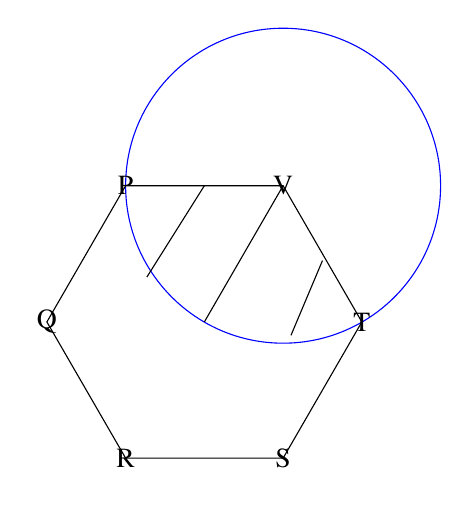
\begin{tikzpicture}
            \draw[blue] (2,3.46) circle (2);
            \draw(1,3.46)--(0.27,2.3);
            \draw(2,3.46)--(1,1.73);
            \draw(2.5,2.509)--(2.1,1.56);
        \draw (0,0) -- (2,0) -- (3,1.73) -- (2,3.46) -- (0,3.46) -- (-1,1.73) -- cycle;
        \node at (0,0) {R};
        \node at (2,0) {S};
        \node at (3,1.73) {T};
        \node at (2,3.46) {V};
        \node at (0,3.46) {P};
        \node at (-1,1.73) {Q};
    \end{tikzpicture}
    \end{center}  
    \end{figure}
    \begin{enumerate}
        \item 5
        \item 10
        \item 8
        \item 9
    \end{enumerate}
    \item A solid spherical bead of lead (uniform density $11000$ kg/m$^3$) of diameter $d = 0.1$ mm sinks with a constant velocity $V$ in a large stagnant pool of a liquid (dynamic viscosity $1.1 \times 10^{-3}$ kg$\cdot$m$^{-1}\cdot$s$^{-1}$). The coefficient of drag is given by $c_D = \frac{24}{\text{Re}}$, where the Reynolds number ($\text{Re}$) is defined on the basis of the diameter of the bead. The drag force acting on the bead is expressed as $D = c_D \left(0.5 \rho V^2 \cdot \frac{\pi d^2}{4}\right)$, where $\rho$ is the liquid density of the liquid. Neglect the buoyancy force,using $g = 10$ m/s$^2$, the velocity $V$ is:
    \begin{enumerate}
        \item $\frac{1}{24}$
        \item $\frac{1}{6}$
        \item $\frac{1}{18}$
        \item $\frac{1}{12}$
    \end{enumerate}
    \item Consider steady,one-dimensional compressible flow of gas in a pipe of diameter $1$ m.At one location in the pipe,the density and velocity at one point are $1$ kg/m$^3$ and $100$ m/s, respectively. At a downstream location in the pipe , the velocity is $170$ m/s. If the pressure drop between these two locations is $10$ kPa, the force exerted by the gas on the pipe between these locations is {\underline{\hspace{2cm}}} N.
    \begin{enumerate}
        \item $350\pi^2$
        \item $750\pi$
        \item $1000\pi$
        \item $3000$
    \end{enumerate}
    \item Consider a rod of uniform thermal conductivity with one end ($x = 0$) is insulated and the other end ($x = L$) is exposed to flow of air at temperature $T_\infty$ with a convective heat transfer coefficient $h$.the cylindrical surface of the rod is insulated so that the heat transfer is strictly along the axis of the rod. The rate of internal heat generation per unit volume inside the rod is given as
    $$q = 2 \pi x \cos \left(\frac{\pi x}{L}\right)$$.
    The steady-state temperature at the midpoint of the rod is $T_A$. If the convective heat transfer coefficient increases to $2h$, the temperature at the midpoint will be:
    \begin{enumerate}
        \item $T_A + \frac{qL}{2h}$
        \item $2T_A$
        \item $T_A$
        \item $T_A \left(1 - \frac{qL}{4\pi h} +  \frac{qL}{4h\pi} T_\infty\right)$
    \end{enumerate}
    \item The system of linear equations in real $(x, y)$ is given by:
\[
    \begin{bmatrix}
        x & y  
    \end{bmatrix}
    \begin{bmatrix} 2 & 5-2\alpha \\ \alpha & 1 \end{bmatrix} = \begin{bmatrix} 0 & 0 \end{bmatrix}
\]
    involves a real parameter $\alpha$ and has infinitely many non-trivial solutions for special value(s) of $\alpha$. Which one or more of the following options is/are non-trivial solution(s) of $(x, y)$ for these value(s) of $\alpha$?
    \begin{enumerate}
        \item $x = 2$, $y = -2$
        \item $x = -1$, $y = 4$
        \item $x = 1$, $y = 1$
        \item $x = 4$, $y = -2$
    \end{enumerate}
    \item Let a random variable $X$ follow a Poisson distribution such that 
    $$\text{Prob}(X = 1) = \text{Prob}(X = 2)$$.
    The value of $\text{Prob}(X = 3)$
    is {\underline{\hspace{2cm}}}(round off to 2 decimal places).
    \item Consider two vectors:
\[
    \bar{a} = 5\hat{i} + 7\hat{j} + 2\hat{k}, \quad \bar{b} = 3\hat{i} - \hat{j} + 6\hat{k}
\]
    The magnitude of the component of $\bar{a}$ orthogonal to $\bar{b}$ in the plane containing the vectors $\bar{a}$ and $\bar{b}$ is {\underline{\hspace{2cm}}}(round off to 2 decimal places).

    \item A structure, along with the loads applied on it, is shown in the figure. Self-weight of all the members is negligible, and all the pin joints are frictionless. $AE$ is a single member that contains pin $C$.Likewise $BE$ is a single member that contains pin $D$. Members $GI$ and $FH$ are overlapping rigid members. The magnitude of the force carried by member $CI$ is {\underline{\hspace{2cm}}} kN (in integer).
     \begin{figure}[H]
        \centering
        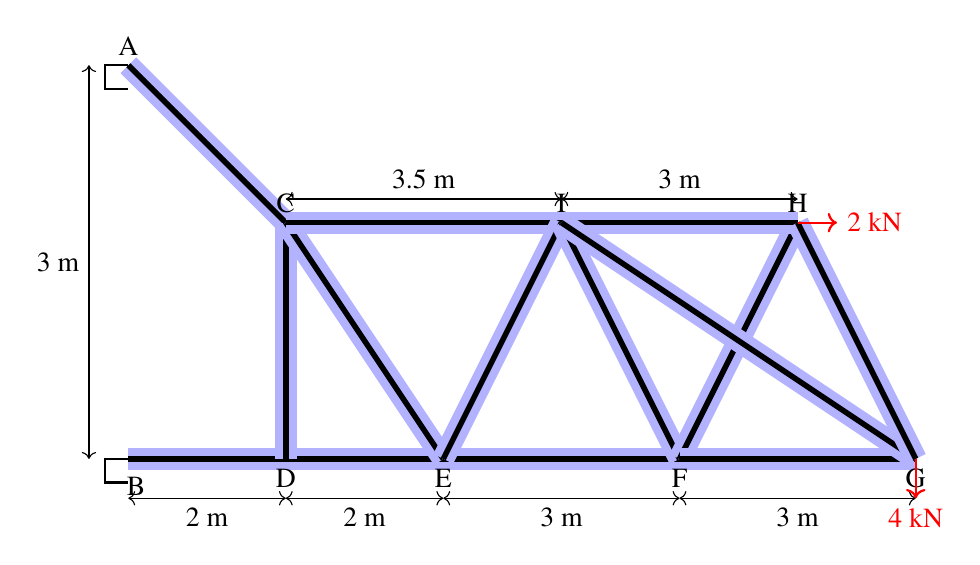
\begin{tikzpicture}
    \coordinate (A) at (0,5);
    \coordinate (B) at (0,0);
    \coordinate (C) at (2,3);
    \coordinate (D) at (2,0);
    \coordinate (E) at (4,0);
    \coordinate (I) at (5.5,3);
    \coordinate (F) at (7,0);
    \coordinate (H) at (8.5,3);
    \coordinate (G) at (10,0);
    \draw[line width=8pt, blue!30] (B) -- (D);
    \draw[line width=2pt, black] (B) -- (D);
    \draw[line width=8pt, blue!30] (D) -- (E);
    \draw[line width=2pt, black] (D) -- (E);
    \draw[line width=8pt, blue!30] (E) -- (F);
    \draw[line width=2pt, black] (E) -- (F);
    \draw[line width=8pt, blue!30] (F) -- (G);
    \draw[line width=2pt, black] (F) -- (G);
    \draw[line width=8pt, blue!30] (A) -- (C);
    \draw[line width=2pt, black] (A) -- (C);
    \draw[line width=8pt, blue!30] (C) -- (D);
    \draw[line width=2pt, black] (C) -- (D);
    \draw[line width=8pt, blue!30] (C) -- (E);
    \draw[line width=2pt, black] (C) -- (E);
    \draw[line width=8pt, blue!30] (C) -- (I);
    \draw[line width=2pt, black] (C) -- (I);
    \draw[line width=8pt, blue!30] (E) -- (I);
    \draw[line width=2pt, black] (E) -- (I);
    \draw[line width=8pt, blue!30] (I) -- (F);
    \draw[line width=2pt, black] (I) -- (F);
    \draw[line width=8pt, blue!30] (F) -- (H);
    \draw[line width=2pt, black] (F) -- (H);
    \draw[line width=8pt, blue!30] (G) -- (F);
    \draw[line width=2pt, black] (G) -- (F);
    \draw[line width=8pt, blue!30] (H) -- (I);
    \draw[line width=2pt, black] (H) -- (I);
    \draw[line width=8pt, blue!30] (I) -- (G);
    \draw[line width=2pt, black] (I) -- (G);
    \draw[line width=8pt, blue!30] (H) -- (G);
    \draw[line width=2pt, black] (H) -- (G);
    \draw[thick] (A) -- ++(-0.3,0) -- ++(0,-0.3) -- ++(0.3,0);
    \draw[thick] (B) -- ++(-0.3,0) -- ++(0,-0.3) -- ++(0.3,0);
    \node[above] at (A) {A};
    \node[below] at (0.1,-0.1) {B};
    \node[above] at (C) {C};
    \node[below] at (D) {D};
    \node[below] at (E) {E};
    \node[above] at (I) {I};
    \node[below] at (F) {F};
    \node[above] at (H) {H};
    \node[below] at (G) {G};
    \draw[<->, thin] (B)++(0,-0.5) -- node[below] {2 m} ++(2,0);
    \draw[<->, thin] (D)++(0,-0.5) -- node[below] {2 m} ++(2,0);
    \draw[<->, thin] (E)++(0,-0.5) -- node[below] {3 m} ++(3,0);
    \draw[<->, thin] (F)++(0,-0.5) -- node[below] {3 m} ++(3,0);
    \draw[<->, thin] (A)++(-0.5,0) -- node[left] {3 m} ++(0,-5);
    \draw[<->, thin] (C)++(0,0.3) -- node[above] {3.5 m} ++(3.5,0);
    \draw[<->, thin] (I)++(0,0.3) -- node[above] {3 m} ++(3,0);
    \draw[red, thick, ->] (H) -- ++(0.5,0) node[right] {2 kN};
    \draw[red, thick, ->] (G) -- ++(0,-0.5) node[below] {4 kN};
\end{tikzpicture}

 
    \end{figure}
    
    \item Two rigid massless rods $PR$ and $RQ$ are joined at a frictionless pin-joint $R$ and are resting on the ground at $P$ and $Q$, respectively, as shown in the figure. A vertical force $F$ acts on pin $R$ as shown. When the included angle $\theta < 90^\circ$, the rods remain in static equilibrium due to Coulomb friction between the rods and ground at locations $P$ and $Q$. At $\theta = 90^\circ$, impending slip occurs simultaneously at points $P$ and $Q$. Then the ratio of the coefficient of friction at $Q$ to that at $P$ $(\mu_Q / \mu_P)$ is {\underline{\hspace{2cm}}} (round off to two decimal places).
     \begin{figure}[H]
        \centering
        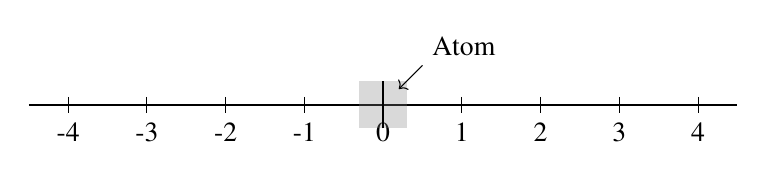
\begin{tikzpicture}
    \draw[thick, -] (-4.5,0) -- (4.5,0);
    \foreach \x in {-4, -3, -2, -1, 0, 1, 2, 3, 4} {
        \draw (\x, 0.1) -- (\x, -0.1);  
        \node[below] at (\x, -0.1) {\x}; 
    }
    \fill[gray, opacity=0.3] (-0.3, -0.3) rectangle (0.3, 0.3);
    \draw[thick] (0, -0.3) -- (0, 0.3);  
    \draw[->] (0.5, 0.5) -- (0.2, 0.2);
    \node[above right] at (0.5, 0.5) {Atom};
\end{tikzpicture}

  
    \end{figure}
    
    \item A cylindrical disc of mass $m = 1$ kg and radius $r = 0.15$ m was spinning at $\omega = 5$ rad/s when it was placed on a flat horizontal surface and released(refer to the figure). Gravity $g$ acts vertically downwards as shown in the figure. The coefficient of friction between the disc and the surface is finite and positive. Disregarding any other dissipation except that due to friction between the disc and the surface, the horizontal velocity of the center of the disc when it starts rolling without slipping,will be{\underline{\hspace{2cm}}} m/s (round off to 2 decimal places).
     \begin{figure}[H]
        \centering
        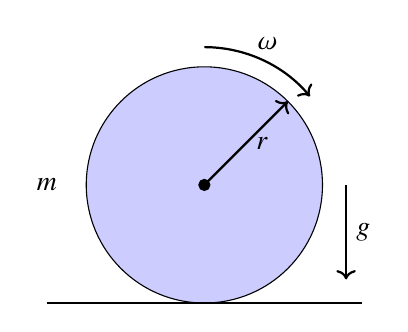
\begin{tikzpicture}
    \fill[blue!20] (0,0) circle (1.5cm); 
    \draw (0,0) circle (1.5cm); 
    \draw[->, thick] (0,0) -- (45:1.5cm) node[midway, right] {$r$};
    \draw[fill=black] (0,0) circle (2pt); 
    \node at (-2, 0) {$m$};
    \draw[->, thick] (0,1.75) arc[start angle=90, end angle=40, radius=1.75cm];
    \node at (0.8,1.8) {$\omega$};
    \draw[thick] (-2, -1.5) -- (2, -1.5); 
    \draw[->, thick] (1.8,0) -- (1.8, -1.2) node[midway, right] {$g$};
\end{tikzpicture}


    \end{figure}
    
    \item A thin-walled cylindrical pressure vessel has mean wall thickness $t$ and nominal radius $r$. The Poisson's ratio of the wall material is $\frac{1}{3}$. When it was subjected to some internal pressure, its nominal perimeter in the cylindrical portion increased by $0.1\%$, and the corresponding wall thickness became $\bar{t}$. The corresponding change in wall thickness of the cylindrical portion, i.e., $100 \times \frac{(t' - t)}{t}$, is {\underline{\hspace{2cm}}}\% (round off to 3 decimal places).
\end{enumerate}
\end{document}